\subsection{Flash Loans}
Flash loans are loans with zero-risk to the liquidity provider\footnote{Ignoring
smart contract bugs, and vulnerabilities}, which enables anyone to borrow large
amounts of money, without any collateral, as long as they pay the loan
back within the same transaction. This will sound crazy to the uninitiated but
let's explain. Usually, there is a risk in lending money, that is, the risk that
the borrower will not pay it back, however, this can be guaranteed by the
blockchain. When a transaction is being executed it can be rolled back if
something invalidates the transaction. So if we say that not repaying the loan
violates the contract, then the block will rollback to before the
transaction.\\

When taking a flash loan you borrow from a liquidity pool, and when borrowing
from this pool you pay back a fee thereby incentivizing individuals and
investors to deposit into the pool.

\subsection{Decentralized exchange (DEX)}
A decentralized exchange is (like normal exchanges) a service where actors can
exchange their assets in a decentralized fashion.

\subsubsection{Limit order book (LOB)}
\begin{wrapfigure}{r}{5.5cm}
  \centering
  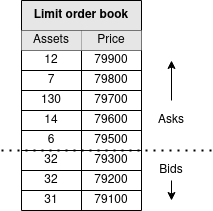
\includegraphics[width=0.3\textwidth]{assests/Flash-loans-LOB}
  \caption{A visual example of a limit order book.}
  \label{fig:LOB}
\end{wrapfigure}
A limit order book is a record of so-called \textit{limit orders}. A limit order
is a trader requesting to buy an asset at up to a certain price or sell an
asset at a minimum specified price. So if we want to sell an asset, an example of
a limit order could be that we want to sell asset X at 15\$ or higher, or if we
were buying we would say that we want to buy asset X at 15\$ or below. A LOB is
simply a record of such limit orders. An example of this can be seen in figure
\ref{fig:LOB}

\subsubsection{Automated market maker (AMM)}
We have specifically looked at Uniswap when understanding AMMs, so while this
background will fit most AMMs, the math/implementation might differ slightly
from AMM to AMM.

AMM's works by exchanging assets between pools in a contract. For example, one
contract could exchange DAI for BTC. This contract will contain a liquidity pool
of DAI and a pool of BTC. This is how Uniswap version 2 works, with a contract
for each exchange pair, ie. a many-to-many relation. Version 1 of Uniswap worked
by having ETH as the to-between currency, meaning that for each asset (X) there
was a contract, containing ETH and X. You could then exchange ETH to X and X to
ETH, but if you wanted to swap Y for X you would need to swap Y for ETH, and ETH
for X. This is not good since you trade twice, and incur the fees associated
with that twice, as well as experiencing the \textit{slippage} in both trades,
and this is one of the things that the second version of the Uniswap protocol fixes.

\paragraph{Price calculation}
Unlike LOBs, it is not immediately clear, what the price of exchanging will be.
The basic formula is $p_t=\frac{r^A_t}{r^B_t}$ \cite[eq 1, page 2]{uniswap},
which means that the price of asset $A$ in terms of asset $B$ at time $t$
($p_t$) is the amount of $A$'s in the contract at time $t$ (reserve $r^A_t$),
divided by the amount of $B$'s in the contract at time $t$ (reserve $r^B_t$).
But this only tells part of the story, since it only describes the price for an
infinitesimal amount of the asset. In reality, the amount of $B$ you will receive
for exchanging an amount of $A$, is determined by the product of the 2 reserves,
before and after the exchange. Before the exchange takes place, the product of
the 2 reserves (time omitted), will form a constant: $r^A \cdot r^B = c$. After
the exchange has taken place, this constant must be the same. So let's say that
we want to exchange an amount of $A$, named $x$, thereby adding $x$ to the
reserve of $A$. Since the product of the 2 reserves must remain constant, the
reserve of $B$ will decrease. This is our payout. We have:

\begin{align*}
  (r^A + x) \cdot (r^B - payout) & = r^A \cdot r^B \Leftrightarrow                 \\
  r^B - payout                   & = \frac{r^A \cdot r^B}{r^A + x} \Leftrightarrow \\
  payout                         & = r^B - \frac{r^A \cdot r^B}{r^A + x}
\end{align*}

\paragraph{Slippage}
As we can see in the equation for payout above, the amount we're payed out does
not double, if we double x. Said more generally, the more we try to exchange,
the higher the price we will pay. The first part of what we buy (keep in mind
that this is continuous, not discrete) is cheaper, than the last part we buy.
This is known as slippage. Since this is dependent on the number of reserves in
the contract, slippage will be high if the reserves are not that big, and lower
if the reserves are great.
